\documentclass{standalone}
\usepackage{tikz}
\usepackage{ctex,siunitx}
\usepackage{tkz-euclide}
\usepackage{amsmath}
\usetikzlibrary{patterns, calc}
\usetikzlibrary {decorations.pathmorphing, decorations.pathreplacing, decorations.shapes,}
\begin{document}
\small
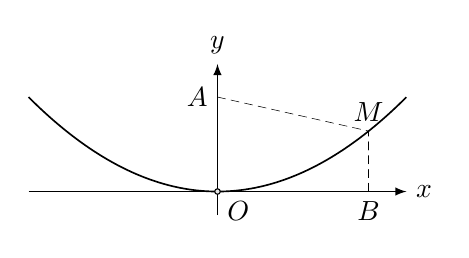
\begin{tikzpicture}[>=latex,scale=0.6,samples=200]
  % \useasboundingbox(0,-0.2)rectangle(3,0.5);
  \draw[thin,->](-4,0)--(4,0)node[right]{$x$};
  \draw[thin,->](0,-0.5)--(0,2.7)node[above]{$y$};
  \draw [semithick,domain=-4:4]  plot (\x,{0.125*\x*\x});
  \tkzDefPoints{0/2/A,3.2/0/B,3.2/1.28/M,0/0/O}
  \tkzDrawSegments[densely dashed](A,M B,M)
  \tkzLabelPoints[left](A)
  \tkzLabelPoints[above](M)
  \tkzLabelPoints(B)
  \tkzDrawPoints(O)
  \tkzLabelPoints[below right](O)
\end{tikzpicture}
\end{document}